%==============================================================
%  Writing / Formatting a Research Article
%  A 6-hour lecture + hands-on workshop for graduate students
%  Running example: Incoming Tourist Trends in Thailand
%  Beamer slide set  --  custom clean "Chula-style" theme
%==============================================================
\documentclass[aspectratio=169,11pt]{beamer}

%------------------------- packages ---------------------------
\usepackage[utf8]{inputenc}
\usepackage[T1]{fontenc}
\usepackage{lmodern}
\usepackage{helvet}
\renewcommand{\familydefault}{\sfdefault}
\usepackage{xcolor}
\usepackage{listings}
\usepackage{booktabs}
\usepackage{tikz}
\usepackage{ragged2e}
\usetikzlibrary{shapes.geometric,arrows.meta,positioning}

%------------------------- colours ----------------------------
\definecolor{chulapink}{RGB}{199,21,133}
\definecolor{chulapinkdk}{RGB}{140,10,95}
\definecolor{inkgray}{RGB}{55,55,60}
\definecolor{softbg}{RGB}{246,238,243}

%------------------------- theme ------------------------------
\usecolortheme{default}
\setbeamertemplate{navigation symbols}{}
\setbeamercolor{normal text}{fg=inkgray}
\setbeamercolor{structure}{fg=chulapink}
\setbeamercolor{title}{fg=chulapinkdk}
\setbeamercolor{frametitle}{fg=chulapinkdk,bg=white}
\setbeamercolor{itemize item}{fg=chulapink}
\setbeamercolor{itemize subitem}{fg=chulapink}
\setbeamercolor{enumerate item}{fg=chulapink}
\setbeamercolor{block title}{fg=white,bg=chulapink}
\setbeamercolor{block body}{fg=inkgray,bg=softbg}
\setbeamercolor{alerted text}{fg=chulapinkdk}
\setbeamercolor{footcolor}{fg=inkgray,bg=softbg}

\setbeamerfont{frametitle}{series=\bfseries,size=\large}
\setbeamerfont{title}{series=\bfseries,size=\Large}
\setbeamerfont{block title}{series=\bfseries}

% bullets
\setbeamertemplate{itemize item}{\textbullet}
\setbeamertemplate{itemize subitem}{--}

% frame title with thin pink rule
\setbeamertemplate{frametitle}{%
  \vskip0.8em
  \begin{beamercolorbox}[leftskip=0.4cm,wd=\paperwidth]{frametitle}%
    \usebeamerfont{frametitle}\insertframetitle%
  \end{beamercolorbox}%
  \vskip2pt{\color{chulapink}\hrule height 1.2pt}\vskip2pt
}

% footline
\setbeamertemplate{footline}{%
  \leavevmode\hbox{%
  \begin{beamercolorbox}[wd=\paperwidth,ht=2.6ex,dp=1.1ex,leftskip=.4cm,rightskip=.4cm]{footcolor}%
    \usebeamerfont{title in head/foot}%
    \insertshorttitle\hfill\insertshortauthor\hfill\insertframenumber\,/\,\inserttotalframenumber%
  \end{beamercolorbox}}%
}

% section divider pages
\setbeamertemplate{section page}{%
  \begin{centering}\vfill
    {\color{chulapink}\hrule height 1.2pt}\vskip1em
    {\usebeamerfont{title}\color{chulapinkdk}\insertsectionhead\par}
    \vskip1em{\color{chulapink}\hrule height 1.2pt}
  \vfill\end{centering}
}
\AtBeginSection[]{\begin{frame}[plain,noframenumbering]\sectionpage\end{frame}}

%------------------------- listings ---------------------------
\lstdefinestyle{tex}{
  basicstyle=\ttfamily\scriptsize,
  keywordstyle=\color{chulapink}\bfseries,
  commentstyle=\color{gray}\itshape,
  stringstyle=\color{teal},
  backgroundcolor=\color{softbg},
  frame=single,framerule=0pt,framesep=6pt,
  breaklines=true,columns=fullflexible,
  showstringspaces=false,keepspaces=true,xleftmargin=4pt,
}
\lstset{style=tex}

%------------------------- metadata ---------------------------
\title[Writing a Research Article]{Writing \& Formatting a Research Article}
\subtitle{Running example: Incoming Tourist Trends in Thailand}
\author[2022517]{Dittaya Wanvarie}
\institute{Chulalongkorn University}
\date{2022517 \,\textbullet\, 2026-06-21}

% handy macros
\newcommand{\faLabel}{\textbf{[LAB]}~}
\newcommand{\lab}[1]{\begin{block}{\faLabel Hands-on Lab}#1\end{block}}
\newcommand{\tipbox}[1]{\begin{block}{Tip}#1\end{block}}

\begin{document}

%================= TITLE =================
\begin{frame}[plain,noframenumbering]
  \vfill
  {\color{chulapink}\hrule height 2pt}\vskip1em
  {\usebeamerfont{title}\color{chulapinkdk}\inserttitle\par}
  \vskip0.4em
  {\large\color{inkgray}\insertsubtitle\par}
  \vskip1em{\color{chulapink}\hrule height 2pt}
  \vskip1.5em
  {\insertauthor\\[0.3em]\insertinstitute\\[0.3em]\insertdate}
  \vfill
\end{frame}

%================= AGENDA =================
\begin{frame}{Today's schedule (09:00--16:00)}
  \begin{columns}[T]
    \begin{column}{0.5\textwidth}
      \footnotesize
      \textbf{Morning}\\[0.3em]
      \begin{tabular}{@{}ll@{}}
        \textbf{09:00} & Welcome \& overview \\
        \textbf{09:15} & 1. Finding a good venue \\
        \textbf{09:55} & \emph{morning break} \\
        \textbf{10:10} & 2. LaTeX \& Overleaf \\
        \textbf{11:05} & 3. Anatomy of an article \\
        \textbf{11:20} & 4. Literature review (1) \\
        \textbf{12:00} & \emph{lunch} \\
      \end{tabular}
    \end{column}
    \begin{column}{0.5\textwidth}
      \footnotesize
      \textbf{Afternoon}\\[0.3em]
      \begin{tabular}{@{}ll@{}}
        \textbf{13:00} & 4. Lit.\ review (2) + refs \\
        \textbf{13:35} & 5. References \& BibTeX \\
        \textbf{14:00} & 6. AI for code \& tables \\
        \textbf{14:30} & \emph{afternoon break} \\
        \textbf{14:45} & 7. AI for figures \\
        \textbf{15:20} & 8. Equations in LaTeX \\
        \textbf{15:40} & 9. Paper $\rightarrow$ Beamer \\
        \textbf{15:55} & Wrap-up \& Q\&A \\
      \end{tabular}
    \end{column}
  \end{columns}
\end{frame}

\begin{frame}{Learning objectives}
  By the end of today you will be able to:
  \begin{itemize}
    \item Choose a suitable venue and read its timelines (time-to-first-decision, deadlines).
    \item Set up an Overleaf project from a publisher template.
    \item Recognise the standard sections of a research article and write each one.
    \item Run a literature review and export it into a reference database.
    \item Manage citations with BibTeX/BibLaTeX.
    \item Use AI to generate LaTeX code and convert spreadsheet results into tables.
    \item Use AI to produce charts and diagrams and import them cleanly into your article.
    \item Typeset equations (e.g.\ the Gaussian PDF) with proper math rendering.
    \item Reuse manuscript content (equations, tables, figures) in Beamer slides.
  \end{itemize}
\end{frame}

%================= RUNNING EXAMPLE =================
\begin{frame}{Our running example: Thai inbound tourism}
  We build \emph{one} short paper from \emph{one} dataset all day.
  \begin{itemize}
    \item \textbf{Working title:} ``Incoming Tourist Trends in Thailand, 2017--2024: Collapse and Recovery.''
    \item \textbf{Data:} \texttt{tourist-data.xlsx} --- two sheets:
    \begin{itemize}
      \item \texttt{Tourist-Number-Data}: arrivals by nationality \& region, 2017--2024.
      \item \texttt{Tourist-Expense-Data}: total \& medical spending, 2017--2023.
    \end{itemize}
    \item \textbf{The story in the numbers:} \textbf{39.9M} arrivals in 2019 $\rightarrow$ \textbf{0.51M} in 2021 (COVID-19) $\rightarrow$ \textbf{35.5M} by 2024.
    \item \textbf{Top source markets (2024):} China, Malaysia, India, South Korea.
  \end{itemize}
  \tipbox{Every module's lab advances this same paper. Follow the printed worksheet step by step.}
\end{frame}

\begin{frame}{The publishing pipeline at a glance}
  \centering
  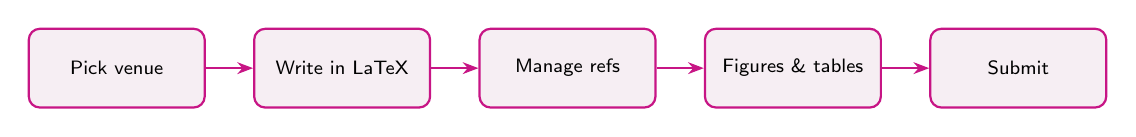
\begin{tikzpicture}[node distance=8mm and 6mm,
      box/.style={draw=chulapink,thick,rounded corners,fill=softbg,
        text width=2.0cm,align=center,minimum height=1.0cm,font=\scriptsize},
      arr/.style={-{Stealth[length=2mm]},chulapink,thick}]
    \node[box](v){Pick venue};
    \node[box,right=of v](w){Write in LaTeX};
    \node[box,right=of w](r){Manage refs};
    \node[box,right=of r](f){Figures \& tables};
    \node[box,right=of f](s){Submit};
    \draw[arr](v)--(w); \draw[arr](w)--(r);
    \draw[arr](r)--(f); \draw[arr](f)--(s);
  \end{tikzpicture}
  \vskip1em
  \footnotesize Today follows exactly this order, module by module.
\end{frame}

%==========================================================
\section{1. Finding a Good Venue}
%==========================================================
\begin{frame}{Why venue choice matters}
  \begin{itemize}
    \item The ``best'' venue is the one whose \textbf{scope, audience, and timeline} fit your paper and your deadlines.
    \item A wrong fit means desk rejection after weeks of waiting --- lost time.
    \item Two big families with different rhythms:
    \begin{itemize}
      \item \textbf{Journals} --- rolling submission, longer review, archival.
      \item \textbf{Conferences} --- fixed deadlines, fast decisions, presentation.
    \end{itemize}
  \end{itemize}
\end{frame}

\begin{frame}{Journal vs. conference: rhythm}
  \centering\footnotesize
  \begin{tabular}{@{}lll@{}}
    \toprule
     & \textbf{Journal} & \textbf{Conference} \\
    \midrule
    Submission & Any time (rolling) & Hard deadline \\
    Decision speed & Weeks to months & Often weeks \\
    Revision & Major/minor rounds & Usually camera-ready only \\
    Output & Archival paper & Talk/poster + proceedings \\
    Page limit & Flexible & Strict \\
    \bottomrule
  \end{tabular}
  \vskip1em
  \justifying For our tourism paper, candidate \emph{journals} (e.g., \emph{Tourism Management}, \emph{Annals of Tourism Research}, \emph{Current Issues in Tourism}) and tourism/Asia-Pacific \emph{conferences} are both reasonable. Know your field's norm.
\end{frame}

\begin{frame}{Reading the timelines}
  \begin{itemize}
    \item \textbf{Time to first decision} --- median weeks from submission to the first editorial decision. Often printed on the journal's ``About'' page.
    \item \textbf{Time to publication} --- acceptance to online/print.
    \item \textbf{Acceptance rate} --- selectivity signal.
    \item \textbf{Conference dates to track:} abstract deadline, full-paper deadline, rebuttal window, notification, camera-ready, event date.
  \end{itemize}
  \tipbox{Work \emph{backwards} from the deadline. Camera-ready is usually only 2--4 weeks after notification --- leave room for it.}
\end{frame}

\begin{frame}{Where to find candidate venues}
  \begin{itemize}
    \item Journal Finder tools (Elsevier, Springer, Taylor \& Francis, Wiley) --- paste title + abstract, get matches.
    \item Conference trackers: WikiCFP, conference-ranking lists (CORE for CS), society websites.
    \item Look at where your \textbf{key references} were published --- that is your community.
    \item Metrics for orientation only: Impact Factor, CiteScore, h5-index, SJR quartile.
  \end{itemize}
\end{frame}

\begin{frame}{Avoiding predatory \& mismatched venues}
  \begin{itemize}
    \item Red flags: spam invitations, promises of ``review in 72 hours'', unclear fees, fake metrics, no real editorial board.
    \item Check: Is it indexed (Scopus, Web of Science, DOAJ)? Is the publisher reputable? Does the scope truly match?
    \item Use checklists like \emph{Think.\,Check.\,Submit.}
  \end{itemize}
  \tipbox{If a venue contacts \emph{you} unsolicited and flatters your ``brilliant work,'' be skeptical.}
\end{frame}

\begin{frame}{[LAB] Shortlist a venue for the tourism paper}
  \lab{
  \footnotesize Spend 20 minutes (Worksheet Step 1):
  \begin{enumerate}
    \item Use a Journal Finder \emph{or} WikiCFP with the title ``\emph{Incoming Tourist Trends in Thailand, 2017--2024}'' + the sample abstract.
    \item Pick \textbf{3 candidate venues} (tourism / hospitality / Asia-Pacific).
    \item For each, record: scope fit (1--5), time-to-first-decision, next deadline, acceptance rate, indexing.
    \item Note the camera-ready / revision window.
  \end{enumerate}
  Deliverable: a 3-row comparison table you reuse later.}
\end{frame}

%==========================================================
\section{2. LaTeX \& Overleaf}
%==========================================================
\begin{frame}{Why LaTeX for research writing}
  \begin{itemize}
    \item Separates \textbf{content} from \textbf{formatting} --- you write, the template styles.
    \item Excellent math, cross-references, figures, tables, and bibliographies.
    \item Publisher templates produce submission-ready output.
    \item Plays well with version control and reproducible workflows.
  \end{itemize}
  \tipbox{LaTeX is a markup language; \textbf{Overleaf} is a browser-based editor that compiles it for you --- no local install.}
\end{frame}

\begin{frame}[fragile]{A minimal LaTeX document}
\begin{lstlisting}[language={[LaTeX]TeX}]
\documentclass[11pt]{article}
\usepackage{graphicx}   % figures
\usepackage{booktabs}   % nice tables
\title{Incoming Tourist Trends in Thailand, 2017--2024}
\author{A. Student}
\begin{document}
\maketitle
\section{Introduction}
Thai inbound arrivals peaked at 39.9 million in 2019.
\end{document}
\end{lstlisting}
  \footnotesize Document = \emph{preamble} (setup, before \verb|\begin{document}|) + \emph{body} (content).
\end{frame}

\begin{frame}[fragile]{Core building blocks}
\begin{lstlisting}[language={[LaTeX]TeX}]
\section{...}  \subsection{...}      % structure
\label{sec:data}  \ref{sec:data}     % cross-reference
\begin{figure}[t]
  \centering
  \includegraphics[width=.6\linewidth]{arrivals.pdf}
  \caption{Arrivals, 2017--2024.}\label{fig:arrivals}
\end{figure}
\begin{table}[t] ... \end{table}
\end{lstlisting}
  \footnotesize Refer to them in text: ``see Fig.~\verb|\ref{fig:arrivals}|''. Numbering updates automatically.
\end{frame}

\begin{frame}{Overleaf in practice}
  \begin{itemize}
    \item Create project: \emph{New Project} $\rightarrow$ upload a template or a \texttt{.zip}.
    \item Left = file tree, middle = source, right = live PDF preview.
    \item \textbf{Recompile} to refresh; errors show in the log panel.
    \item \textbf{Share} for real-time co-authoring; \textbf{History} tracks versions.
    \item Set the compiler (pdfLaTeX / XeLaTeX) and main document in \emph{Menu}.
  \end{itemize}
\end{frame}

\begin{frame}{Using a publisher template}
  \begin{enumerate}
    \item Find it: Overleaf Template Gallery, or download from the journal/conference site (e.g., \texttt{elsarticle}, Springer \texttt{sn-jnl}, Taylor \& Francis \texttt{interact}).
    \item Open in Overleaf $\rightarrow$ \emph{don't} fight the style; fill in the placeholders.
    \item Replace title, authors, abstract; keep the document class options the venue requires.
    \item Read the template's own comments --- they tell you what each field expects.
  \end{enumerate}
  \tipbox{Never change margins/fonts to ``save space.'' Reviewers and editors notice, and it can get you desk-rejected.}
\end{frame}

\begin{frame}{[LAB] Build your project on a real template}
  \lab{
  \footnotesize 30 minutes (Worksheet Step 2):
  \begin{enumerate}
    \item Open Overleaf; start from the template of the venue you shortlisted in Module 1.
    \item Fill in the title and authors; paste the sample tourism abstract.
    \item Add sections: Introduction, Data, Results, Discussion --- plus a figure and a table placeholder.
    \item Compile to a clean PDF; fix any errors from the log.
  \end{enumerate}
  Keep this project open --- we add references, tables, and figures to it all afternoon.}
\end{frame}

%==========================================================
\section{3. Anatomy of a Research Article}
%==========================================================
\begin{frame}{The standard sections (IMRaD)}
  Most empirical papers share the same skeleton:
  \begin{itemize}
    \item \textbf{Title \& Abstract} --- what the paper is, in one breath.
    \item \textbf{Introduction} --- the problem, the gap, your contribution.
    \item \textbf{Related Work / Literature Review} --- situate the paper against prior work (this is where you \emph{cite}).
    \item \textbf{Data / Materials \& Methods} --- what you used and what you did.
    \item \textbf{Results} --- the findings, shown with tables \& figures.
    \item \textbf{Discussion} --- interpretation, implications, limitations.
    \item \textbf{Conclusion} --- takeaways and future work.
    \item \textbf{References} --- every source you cited.
  \end{itemize}
  \footnotesize Names and order vary by field and venue.
\end{frame}

\begin{frame}{We build it section by section}
  How our tourism paper maps onto the skeleton --- and onto today:
  \begin{itemize}
    \item \textbf{Introduction \& Literature Review} --- next: search and cite prior work.
    \item \textbf{Data} --- \texttt{tourist-data.xlsx} and how it was collected.
    \item \textbf{Results} --- the arrivals table (Module 6) and chart (Module 7).
    \item \textbf{References} --- the bibliography and its style (Module 5).
  \end{itemize}
  \tipbox{A common drafting order is \textbf{Methods $\rightarrow$ Results $\rightarrow$ Introduction $\rightarrow$ Abstract} --- write the factual parts first.}
\end{frame}

%==========================================================
\section{4. The Literature Review}
%==========================================================
\begin{frame}{Goals of a literature review}
  \begin{itemize}
    \item Map the field: what is known, what is contested, where the gap is.
    \item Justify your contribution and method choices.
    \item Build a reusable, well-organized \textbf{reference database} --- not a pile of PDFs.
  \end{itemize}
\end{frame}

\begin{frame}{Searching effectively}
  \begin{itemize}
    \item Start broad on Google Scholar / Scopus / Web of Science / your field's database.
    \item Use \textbf{Boolean} queries and synonyms; record the queries you ran.
    \item \textbf{Snowballing}: follow citations backward (references) and forward (cited-by).
    \item Visual discovery: Connected Papers, Litmaps, ResearchRabbit show citation networks.
    \item Track screening decisions (include/exclude + reason) for transparency.
  \end{itemize}
\end{frame}

\begin{frame}{Discovery tools: Google Scholar \& ResearchRabbit}
  \textbf{Google Scholar} --- broad, free index across publishers.
  \begin{itemize}
    \item ``Cited by'' for forward snowballing; ``Related articles''.
    \item Set up \emph{Alerts} for new papers matching your query.
    \item One-click \emph{Cite} $\rightarrow$ \textbf{BibTeX}; \emph{Save} to ``My library''.
  \end{itemize}
  \textbf{ResearchRabbit} --- free, visual ``Spotify for papers''.
  \begin{itemize}
    \item Start from a few seed papers; get recommendations and citation / co-author networks.
    \item Build collections and \textbf{sync directly with Zotero}.
  \end{itemize}
\end{frame}

\begin{frame}{AI tools: AIX at the library vs. free versions today}
  Chula's Central Library (\textbf{AIX}) subscribes to premium tiers of several AI tools --- but these are \textbf{usable on-site at the library only}.
  \begin{itemize}
    \item \textbf{For literature review:} Consensus, Connected Papers, SciSpace.
    \item \textbf{General assistants:} ChatGPT, Claude, Gemini.
    \item \textbf{Writing \& media:} Grammarly, Runway.
  \end{itemize}
  \tipbox{See the list at \texttt{aix.car.chula.ac.th} (``Subscribed AI Tools''). \textbf{For today's workshop, just sign up for the free version of each tool with any account} --- the free tiers cover every lab.}
\end{frame}

\begin{frame}{AI tools for finding \& understanding papers}
  \begin{itemize}
    \item \textbf{Consensus} --- ask a research question in plain language; returns an evidence-based synthesis with citations to real papers. Good for ``\emph{Has Thai tourism recovered post-COVID?}''
    \item \textbf{Connected Papers} --- enter a seed paper; get a visual graph of related work to spot foundational and derivative papers fast.
    \item \textbf{SciSpace} --- ``chat with PDF''; extract methods, datasets, and results; build comparison tables across papers; explain difficult passages.
  \end{itemize}
  \alert{Always open and read the real paper} --- these tools point you to evidence; they do not replace reading it.
\end{frame}

\begin{frame}{NotebookLM: draft the review from your sources}
  Upload your shortlisted PDFs as \textbf{sources}; NotebookLM answers \emph{only} from them, with inline citations.
  \begin{itemize}
    \item \textbf{Extract keys per paper:} ``\emph{For each source, list the research question, method, data, and main finding.}''
    \item \textbf{Find themes:} ask it to group papers by topic and surface agreements / contradictions.
    \item \textbf{Draft an outline:} ask for a literature-review structure with the sources mapped to each subsection.
  \end{itemize}
  \tipbox{Grounded in your uploads = fewer hallucinations --- but you still verify quotes and never let it write claims you have not checked.}
\end{frame}

\begin{frame}{Reference managers}
  \centering\footnotesize
  \begin{tabular}{@{}llll@{}}
    \toprule
     & \textbf{Zotero} & \textbf{Mendeley} & \textbf{EndNote} \\
    \midrule
    Cost & Free/open & Free & Paid \\
    Browser capture & Excellent & Good & Good \\
    PDF + notes & Yes & Yes & Yes \\
    BibTeX export & Native (Better BibTeX) & Yes & Yes \\
    Best for & Most grad students & Elsevier users & Institutions \\
    \bottomrule
  \end{tabular}
  \vskip1em
  \justifying A manager is \textbf{optional} --- great for big projects, but you can also grab BibTeX directly (next slide). Any of these can output the \texttt{.bib} file LaTeX needs.
\end{frame}

\begin{frame}{Optional: capturing references with a manager}
  If you choose to use Zotero / Mendeley:
  \begin{itemize}
    \item Install the browser connector; one click saves the item + PDF + metadata.
    \item Import by DOI / ISBN / PubMed ID when metadata is missing.
    \item Organize with \textbf{collections} (per project) and \textbf{tags} (per theme).
    \item \textbf{Clean as you go:} fix author names, titles, and that all-important \emph{cite key}.
  \end{itemize}
  \tipbox{Garbage in, garbage out --- a messy library produces messy citations. Five minutes of cleanup now saves an hour at submission.}
\end{frame}

\begin{frame}{Get BibTeX directly --- no manager required}
  \begin{itemize}
    \item \textbf{Google Scholar:} click \emph{Cite} $\rightarrow$ \emph{BibTeX} and copy the entry straight into \texttt{references.bib}.
    \item \textbf{Publisher / DOI pages \& Crossref:} most offer ``Export citation $\rightarrow$ BibTeX''.
    \item \textbf{NotebookLM / SciSpace:} ask for the BibTeX of each source, then verify it.
    \item \textbf{Zotero (optional):} right-click collection $\rightarrow$ \emph{Export} $\rightarrow$ \emph{BibTeX} --- best when you have many papers.
    \item Keep \emph{one} \texttt{references.bib}; paste new entries as you find them.
  \end{itemize}
  \alert{Always check} each entry: authors, title capitals, year, DOI.
\end{frame}

\begin{frame}[fragile]{Cite as you write: \texttt{\textbackslash cite} + references.bib}
\begin{lstlisting}[language={[LaTeX]TeX}]
% references.bib holds the entries; you cite by KEY:
Arrivals rebounded strongly by 2024 \cite{chen2022recovery}.
Several studies note an uneven recovery
  \cite{kim2021pandemic, li2020china}.
\end{lstlisting}
  \footnotesize Cite \emph{while} you read, not at the end. \texttt{\textbackslash cite\{key\}} inserts the in-text marker and adds the work to the reference list automatically.
  \tipbox{How citations \emph{look} (numbers vs.\ author--year) is set by the \texttt{bibliographystyle} --- covered later in the References section (Module 5).}
\end{frame}

\begin{frame}[fragile]{Anatomy of a .bib entry}
\begin{lstlisting}
@article{chen2022recovery,
  author  = {Chen, Mei and Suthida, Pra},
  title   = {Tourism Recovery in {Thailand} after {COVID-19}},
  journal = {Current Issues in Tourism},
  year    = {2022},
  volume  = {25},
  number  = {7},
  pages   = {1021--1039},
  doi     = {10.1080/cit.2022.0107}
}
\end{lstlisting}
  \footnotesize \texttt{@article} = entry type; \texttt{chen2022recovery} = the \textbf{cite key} you pass to \texttt{\textbackslash cite}. \textbf{Protect capitals} in titles with braces: \texttt{\{Thailand\}}, \texttt{\{COVID-19\}}. Other types: \texttt{@inproceedings}, \texttt{@book}, \texttt{@techreport}, \texttt{@misc}.
\end{frame}

\begin{frame}{Ethics of using AI --- the non-negotiables}
  \begin{itemize}
    \item \textbf{You are the author and are accountable.} AI cannot be listed as an author.
    \item \textbf{Never trust AI citations blindly} --- chatbots invent plausible-looking references. Verify every DOI against the real paper.
    \item \textbf{Protect data \& IP} --- do not upload confidential, unpublished, or others' copyrighted material to public tools.
    \item \textbf{No fabrication} --- AI must not generate or alter data, results, or images.
    \item \textbf{Disclose} your AI use as each venue requires.
  \end{itemize}
\end{frame}

\begin{frame}{Each venue has an AI policy --- read it before you submit}
  \footnotesize
  \textbf{Elsevier} (policy updated 2025)
  \begin{itemize}
    \item AI for \emph{language improvement} allowed \emph{with human oversight}; plain grammar / spell-check needs no declaration.
    \item Add a \textbf{disclosure statement} in its own section, immediately before the references.
    \item AI \emph{image} generation / alteration prohibited (unless a documented part of the methodology). AI is not an author.
  \end{itemize}
  \textbf{Taylor \& Francis}
  \begin{itemize}
    \item Disclose the tool's \textbf{name + version, how, and why}, in the \emph{Methods or Acknowledgements}.
    \item Copyediting / idea exploration / language support welcomed; \emph{image} \& figure generation not permitted. AI is not an author.
  \end{itemize}
  \tipbox{Policies differ by publisher \emph{and} change often --- check the ``Guide for Authors'' for your specific venue.}
\end{frame}

\begin{frame}{[LAB] From search to .bib}
  \lab{
  \footnotesize 25 minutes (Worksheet Step 3):
  \begin{enumerate}
    \item Search in \textbf{Google Scholar} (free): ``Thailand inbound tourism'', ``COVID-19 tourism recovery''. Find \textbf{8--10} relevant papers.
    \item Grab BibTeX directly: Scholar \emph{Cite} $\rightarrow$ \emph{BibTeX} (or the DOI page); paste into \texttt{references.bib}.
    \item Expand with \textbf{ResearchRabbit} / \textbf{Connected Papers} (free) from one seed paper.
    \item Upload the PDFs to \textbf{NotebookLM} (free); extract each paper's key points.
    \item Upload \texttt{references.bib} to Overleaf (Zotero optional). \textbf{Check} your venue's AI-disclosure policy.
  \end{enumerate}}
\end{frame}

%==========================================================
\section{5. The References Section}
%==========================================================
\begin{frame}{The References section: built for you}
  \begin{itemize}
    \item You never type the reference list by hand.
    \item BibTeX / BibLaTeX collects every key you \texttt{\textbackslash cite}d, looks it up in \texttt{references.bib}, and builds the list in the required \textbf{style}.
    \item Change venues $\rightarrow$ change one line $\rightarrow$ the whole list reformats.
  \end{itemize}
\end{frame}

\begin{frame}[fragile]{Setting the style: \texttt{\textbackslash bibliographystyle}}
\begin{lstlisting}[language={[LaTeX]TeX}]
% choose the style (preamble or before the list):
\bibliographystyle{apalike}   % plain, abbrv, ieeetr,
                              % elsarticle-num, ...
% at the end of the document:
\bibliography{references}      % -> references.bib
\end{lstlisting}
  \footnotesize The \texttt{bibliographystyle} controls how the citations and the list \emph{look} --- it must match your venue. Compile order: \textbf{pdflatex $\rightarrow$ bibtex $\rightarrow$ pdflatex $\rightarrow$ pdflatex} (Overleaf does this on Recompile).
\end{frame}

\begin{frame}[fragile]{Modern alternative: BibLaTeX + biber}
\begin{lstlisting}[language={[LaTeX]TeX}]
\usepackage[style=authoryear,backend=biber]{biblatex}
\addbibresource{references.bib}
...
Recovery was uneven across source markets \autocite{chen2022recovery}.
...
\printbibliography
\end{lstlisting}
  \footnotesize BibLaTeX is more flexible (Unicode, styles, multiple bibliographies). Use whichever your \textbf{template} expects --- don't mix the two.
\end{frame}

\begin{frame}{Common fixes}
  \begin{itemize}
    \item \texttt{\textbackslash cite}, \texttt{\textbackslash citet} / \texttt{\textbackslash citep} (natbib), \texttt{\textbackslash autocite} (biblatex).
    \item Undefined references? Recompile (and run bibtex / biber) again.
    \item Keep cite keys stable --- Better BibTeX prevents them from changing under you.
    \item Wrong-looking list? Check the \texttt{bibliographystyle} matches the venue.
  \end{itemize}
  \tipbox{Match the \texttt{bibliographystyle} to your venue's required citation style \emph{before} you submit.}
\end{frame}

\begin{frame}{[LAB] Wire up your bibliography}
  \lab{
  \footnotesize 25 minutes (Worksheet Step 4):
  \begin{enumerate}
    \item Add \texttt{references.bib} to your Overleaf project (from Module 4).
    \item Set \texttt{\textbackslash bibliographystyle} to the style your venue requires; add \texttt{\textbackslash bibliography\{references\}}.
    \item Make sure your \textbf{4+} citations resolve; print the reference list.
    \item Recompile until there are \emph{no} undefined-citation warnings.
  \end{enumerate}}
\end{frame}

%==========================================================
\section{6. AI for LaTeX Code \& Tables}
%==========================================================
\begin{frame}{How AI helps with LaTeX}
  \begin{itemize}
    \item Generate boilerplate (environments, TikZ, tables) you would otherwise look up.
    \item Convert \textbf{Excel/CSV results into LaTeX tables} in seconds.
    \item Explain and fix cryptic compiler errors.
    \item Refactor and tidy messy LaTeX.
  \end{itemize}
  \alert{Golden rule:} you are the author. \textbf{Always compile and verify} AI output --- it can invent packages or commands.
\end{frame}

\begin{frame}{Prompting for good LaTeX}
  \begin{itemize}
    \item State the target: ``\emph{Give me a \texttt{booktabs} 3-column table, caption, label \texttt{tab:arrivals}.}''
    \item Give the data and the constraints (column types, units, significant figures).
    \item Ask for \textbf{compilable} code and to list any required packages.
    \item Iterate: paste the error log back and ask for a fix.
  \end{itemize}
  \tipbox{Tell the AI which document class/template you use so it matches your setup.}
\end{frame}

\begin{frame}[fragile]{Example: Excel results to a LaTeX table}
  \footnotesize Copy this pivot from \texttt{tourist-data.xlsx} and ask AI to format it:
\begin{lstlisting}
Year, Arrivals (millions)
2019, 39.92
2021, 0.51
2024, 35.55
\end{lstlisting}
  Typical AI output:
\begin{lstlisting}[language={[LaTeX]TeX}]
\begin{table}[t]\centering
\caption{Thai tourist arrivals, selected years.}\label{tab:arrivals}
\begin{tabular}{lc}
\toprule
Year & Arrivals (millions) \\ \midrule
2019 & 39.92 \\
2021 & \textbf{0.51} \\
2024 & 35.55 \\
\bottomrule
\end{tabular}
\end{table}
\end{lstlisting}
\end{frame}

\begin{frame}{Verifying AI-generated tables}
  \begin{itemize}
    \item Check the \textbf{numbers} against \texttt{tourist-data.xlsx} --- AI may round or transpose.
    \item Confirm column alignment and units (millions vs.\ raw counts); bold only what you mean to highlight.
    \item Make sure \texttt{\textbackslash caption} is above the data and \texttt{\textbackslash label} is set for \texttt{\textbackslash ref}.
    \item Prefer \texttt{booktabs} rules; avoid vertical lines in scientific tables.
  \end{itemize}
  \tipbox{For repeatability, you can also export tables directly from pandas (\texttt{df.to\_latex}) --- AI is fastest for one-off formatting.}
\end{frame}

\begin{frame}{[LAB] Turn the tourist data into a table}
  \lab{
  \footnotesize 25 minutes (Worksheet Step 5):
  \begin{enumerate}
    \item In \texttt{tourist-data.xlsx}, build a pivot of \textbf{total arrivals by year (2017--2024)} \emph{or} the \textbf{top-10 nationalities in 2024}.
    \item Copy it as CSV; ask an AI assistant for a \texttt{booktabs} table with caption + label.
    \item Paste it into Overleaf and compile.
    \item \textbf{Verify every number} against the sheet; cross-reference the table in the text.
  \end{enumerate}}
\end{frame}

%==========================================================
\section{7. AI for Figures, Diagrams \& Graphics}
%==========================================================
\begin{frame}{Figures: what we want}
  \begin{itemize}
    \item \textbf{Vector} graphics (PDF/EPS) for plots and diagrams --- crisp at any zoom.
    \item Readable fonts and labels, colorblind-friendly palettes.
    \item Reproducible: keep the script/source that made each figure.
    \item Consistent sizing and style across the paper.
  \end{itemize}
\end{frame}

\begin{frame}[fragile]{AI for charts from analysis results}
  \footnotesize Ask AI for a plotting script, then run it to export a PDF:
\begin{lstlisting}
# prompt: "matplotlib line chart of Thai tourist arrivals
#          by year 2017-2024, save arrivals.pdf, label axes"
import matplotlib.pyplot as plt
year = [2017,2018,2019,2020,2021,2022,2023,2024]
arr  = [35.6,38.2,39.9,6.7,0.5,11.1,28.2,35.5]  # millions
plt.figure(figsize=(4,3))
plt.plot(year, arr, marker="o")
plt.ylabel("Arrivals (millions)"); plt.xlabel("Year")
plt.tight_layout(); plt.savefig("arrivals.pdf")
\end{lstlisting}
  You keep the script for reproducibility; include the PDF in LaTeX (next slide).
\end{frame}

\begin{frame}{Where to run the code: Google Colab (no install)}
  No Python on your laptop? Use \textbf{Google Colab} --- free, browser-based, nothing to install.
  \begin{itemize}
    \item Open \texttt{colab.research.google.com} $\rightarrow$ \emph{New notebook} (runs on Google's servers).
    \item Upload \texttt{tourist-data.xlsx}, paste the AI-generated script, press \emph{Run}.
    \item Download the resulting \texttt{arrivals.pdf} and drop it into Overleaf.
    \item \texttt{pandas} and \texttt{matplotlib} are already pre-installed.
  \end{itemize}
  \tipbox{Alternatively, ask an AI assistant (e.g.\ NotebookLM / ChatGPT) to generate the plotting code or describe the chart --- but you still run it and \textbf{verify the numbers}.}
\end{frame}

\begin{frame}[fragile]{AI for diagrams (TikZ / Mermaid)}
\begin{lstlisting}[language={[LaTeX]TeX}]
% prompt: "TikZ flowchart: Excel -> Python -> Figure -> LaTeX"
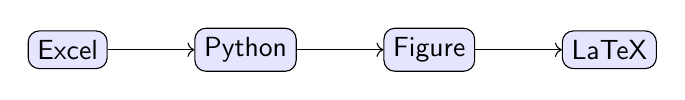
\begin{tikzpicture}[node distance=1.1cm,
  box/.style={draw,rounded corners,fill=blue!10}]
  \node[box](d){Excel};
  \node[box,right=of d](p){Python};
  \node[box,right=of p](f){Figure};
  \node[box,right=of f](l){LaTeX};
  \draw[->](d)--(p); \draw[->](p)--(f); \draw[->](f)--(l);
\end{tikzpicture}
\end{lstlisting}
  \footnotesize TikZ diagrams are vector and editable. AI is great at drafting them; you tweak spacing and labels. Mermaid is an easy alternative you can render to an image.
\end{frame}

\begin{frame}[fragile]{Importing graphics cleanly}
\begin{lstlisting}[language={[LaTeX]TeX}]
\usepackage{graphicx}        % in preamble
...
\begin{figure}[t]\centering
  \includegraphics[width=.7\linewidth]{arrivals.pdf}
  \caption{Thai tourist arrivals, 2017--2024.}\label{fig:arr}
\end{figure}
As Fig.~\ref{fig:arr} shows, arrivals collapsed in 2020--21
and recovered to near-2019 levels by 2024.
\end{lstlisting}
  \footnotesize Use \texttt{width=...\textbackslash linewidth} (not fixed cm) so figures scale to the column. Place files in a \texttt{figures/} folder and reference by name.
\end{frame}

\begin{frame}{Quality \& integrity checklist for figures}
  \begin{itemize}
    \item Every figure is \textbf{referenced} in the text and has a self-contained caption.
    \item Data shown is real and matches \texttt{tourist-data.xlsx} --- never let AI fabricate data points.
    \item Vector where possible; if raster, use high resolution (300+ dpi).
    \item Fonts in the figure are legible at print size; colors distinguishable in grayscale.
  \end{itemize}
  \alert{Integrity:} AI assists with \emph{code and layout}, not with inventing results. Disclose AI use per your venue's policy.
\end{frame}

\begin{frame}{[LAB] Make and import a figure}
  \lab{
  \footnotesize 25 minutes (Worksheet Step 6):
  \begin{enumerate}
    \item Ask AI for a matplotlib script that plots arrivals 2017--2024 (or expense by year) to \texttt{arrivals.pdf}.
    \item Run it; check axes, labels, and that values match the sheet.
    \item \texttt{\textbackslash includegraphics} it into Overleaf; add caption + label.
    \item Cross-reference it in the text and recompile to a clean PDF.
    \item Bonus: draft a TikZ or Mermaid diagram of your data workflow.
  \end{enumerate}}
\end{frame}

%==========================================================
\section{8. Equations in LaTeX}
%==========================================================
\begin{frame}{Why LaTeX wins for equations}
  \begin{itemize}
    \item \textbf{Publication-quality math} --- far better spacing and symbols than a word-processor editor.
    \item \textbf{Numbered \& cross-referenced} --- \texttt{\textbackslash label}/\texttt{\textbackslash eqref} keep equation numbers correct automatically.
    \item \textbf{Consistent notation} --- define a macro once, reuse it everywhere.
    \item \textbf{Portable} --- the same source drops into slides, posters, and reviewer replies.
  \end{itemize}
  \tipbox{Wrap math in \texttt{\$...\$} (inline) or an \texttt{equation} environment (display). Load \texttt{amsmath} for the good stuff.}
\end{frame}

\begin{frame}[fragile]{Example: the Gaussian (normal) PDF}
  \footnotesize Source:
\begin{lstlisting}[language={[LaTeX]TeX}]
\usepackage{amsmath}   % preamble
...
\begin{equation}
  f(x)=\frac{1}{\sigma\sqrt{2\pi}}\,
       \exp\!\left(-\frac{(x-\mu)^2}{2\sigma^2}\right)
  \label{eq:gauss}
\end{equation}
As Eq.~\eqref{eq:gauss} shows, log-arrivals are Gaussian.
\end{lstlisting}
  Renders as:
  \begin{equation*}
    f(x)=\frac{1}{\sigma\sqrt{2\pi}}\,
         \exp\!\left(-\frac{(x-\mu)^2}{2\sigma^2}\right)
  \end{equation*}
\end{frame}

\begin{frame}{[LAB] Typeset the Gaussian analysis}
  \lab{
  \footnotesize 20 minutes (Worksheet Step 7):
  \begin{enumerate}
    \item In Colab, fit a normal to \texttt{ln(arrivals)} for 2024; record $\mu,\sigma$ (about $11.1$ and $2.0$).
    \item Add a \texttt{Methods} section with the Gaussian PDF in an \texttt{equation} environment + \texttt{\textbackslash label}.
    \item Plot the histogram with the fitted curve; save \texttt{gaussian\_fit.pdf} and include it.
    \item Refer to it with \texttt{Eq.~\textbackslash eqref\{eq:gauss\}} and recompile.
  \end{enumerate}}
\end{frame}

%==========================================================
\section{9. From Paper to Slides: Beamer}
%==========================================================
\begin{frame}{Reuse your manuscript as slides}
  \begin{itemize}
    \item Conferences want a \textbf{talk} --- Beamer makes slides from the LaTeX you already wrote.
    \item \textbf{One source of truth:} the same equations, tables, figures, and \texttt{.bib} drop straight in --- no re-typing, no broken math.
    \item Change a result once; update the paper \emph{and} the slides from the same numbers.
    \item \emph{This very deck} is a Beamer document.
  \end{itemize}
  \tipbox{Word $\rightarrow$ PowerPoint usually breaks equations and figures; LaTeX $\rightarrow$ Beamer does not.}
\end{frame}

\begin{frame}[fragile=singleslide]{A minimal Beamer frame (reuse the equation)}
\begin{lstlisting}[language={[LaTeX]TeX}]
\documentclass{beamer}
\usepackage{amsmath}
\begin{document}
\begin{frame}{Log-arrivals are Gaussian}
  \begin{equation*}
    f(x)=\frac{1}{\sigma\sqrt{2\pi}}
         \exp\!\left(-\frac{(x-\mu)^2}{2\sigma^2}\right)
  \end{equation*}
  \includegraphics[width=.6\linewidth]{gaussian_fit.pdf}
\end{frame}
\end{document}
\end{lstlisting}
  \footnotesize The same equation and figure as the paper --- copied verbatim.
\end{frame}

\begin{frame}{[LAB] Make one slide from your paper}
  \lab{
  \footnotesize 20 minutes (Worksheet Step 8):
  \begin{enumerate}
    \item Start a Beamer project on Overleaf (or copy the template provided).
    \item Make one \texttt{frame} that reuses your Gaussian equation and \texttt{gaussian\_fit.pdf}.
    \item Add a second \texttt{frame} with your arrivals table or chart --- copy-paste from the paper.
    \item Compile; note that nothing had to be redrawn.
  \end{enumerate}}
\end{frame}

%==========================================================
\section{Wrap-up}
%==========================================================
\begin{frame}{What you built today}
  One paper on \textbf{Thai inbound tourism}, end to end:
  \begin{itemize}
    \item A shortlist of tourism venues with timelines and deadlines.
    \item An Overleaf project on a real publisher template, with a sample abstract.
    \item A \texttt{references.bib} wired up with BibTeX and a venue-matched style.
    \item AI-assisted arrivals table and chart, verified against the data.
    \item A typeset Gaussian analysis, and a Beamer slide reusing the same equation and figure.
  \end{itemize}
  \tipbox{You now have the skeleton of a submittable manuscript \emph{and} its talk --- keep filling them in.}
\end{frame}

\begin{frame}{Good habits to keep}
  \begin{itemize}
    \item Decide the venue \emph{early}; write to its template and limits.
    \item Capture every reference the moment you read it; clean as you go.
    \item Keep one \texttt{.bib}, stable cite keys, and the scripts that build your figures.
    \item Treat AI as a fast assistant --- \textbf{you verify, you are accountable}.
  \end{itemize}
\end{frame}

\begin{frame}[plain,noframenumbering]
  \vfill\centering
  {\color{chulapink}\hrule height 2pt}\vskip1em
  {\usebeamerfont{title}\color{chulapinkdk}Thank you --- Questions?}\par
  \vskip0.6em{\footnotesize Writing \& Formatting a Research Article --- Thai Inbound Tourism}\par
  \vskip1em{\color{chulapink}\hrule height 2pt}
  \vfill
\end{frame}

\end{document}
